\chapter{Expression des besoins}
\clearpage
\label{chap:besoins}

\section{Introduction}
Lorem ipsum dolor sit amet, consectetur adipiscing elit. Proin posuere euismod neque, non semper nibh viverra sed. Praesent ut varius magna. Fusce ipsum ante, semper nec interdum at, semper et lacus. Nulla ultrices magna a fringilla finibus. Etiam sollicitudin blandit ante. Vivamus blandit rhoncus tincidunt. Morbi sit amet congue purus. Praesent interdum gravida congue. Donec fermentum dui fermentum maximus rutrum.
\section{Définition des utilisateurs}
Lorem ipsum dolor sit amet, consectetur adipiscing elit. Proin posuere euismod neque, non semper nibh viverra sed. Praesent ut varius magna. Fusce ipsum ante, semper nec interdum at, semper et lacus. Nulla ultrices magna a fringilla finibus. Etiam sollicitudin blandit ante. Vivamus blandit rhoncus tincidunt. Morbi sit amet congue purus. Praesent interdum gravida congue. Donec fermentum dui fermentum maximus rutrum.
\subsection{Administrateur}
Lorem ipsum dolor sit amet, consectetur adipiscing elit. Proin posuere euismod neque, non semper nibh viverra sed. Praesent ut varius magna. Fusce ipsum ante, semper nec interdum at, semper et lacus. Nulla ultrices magna a fringilla finibus. Etiam sollicitudin blandit ante. Vivamus blandit rhoncus tincidunt. Morbi sit amet congue purus. Praesent interdum gravida congue. Donec fermentum dui fermentum maximus rutrum.


\subsection{Animateur}
Lorem ipsum dolor sit amet, consectetur adipiscing elit. Proin posuere euismod neque, non semper nibh viverra sed. Praesent ut varius magna. Fusce ipsum ante, semper nec interdum at, semper et lacus. Nulla ultrices magna a fringilla finibus. Etiam sollicitudin blandit ante. Vivamus blandit rhoncus tincidunt. Morbi sit amet congue purus. Praesent interdum gravida congue. Donec fermentum dui fermentum maximus rutrum.

\clearpage

\section{Spécifications}
Lorem ipsum dolor sit amet, consectetur adipiscing elit. Proin posuere euismod neque, non semper nibh viverra sed. Praesent ut varius magna. Fusce ipsum ante, semper nec interdum at, semper et lacus. Nulla ultrices magna a fringilla finibus. Etiam sollicitudin blandit ante. Vivamus blandit rhoncus tincidunt. Morbi sit amet congue purus. Praesent interdum gravida congue. Donec fermentum dui fermentum maximus rutrum.

\subsection{Spécifications fonctionnelles}
Lorem ipsum dolor sit amet, consectetur adipiscing elit. Proin posuere euismod neque, non semper nibh viverra sed. Praesent ut varius magna. Fusce ipsum ante, semper nec interdum at, semper et lacus. Nulla ultrices magna a fringilla finibus. Etiam sollicitudin blandit ante. Vivamus blandit rhoncus tincidunt. Morbi sit amet congue purus. Praesent interdum gravida congue. Donec fermentum dui fermentum maximus rutrum. :
\renewcommand{\arraystretch}{1.5}
\begin{xltabular}{17cm}{|c|X|}
    \hline
    ID & Description     \\\hline
    1 & Le système doit permettre à l'utilisateur (Administrateur, Animateur) de s'authentifier. \\\hline
    2 & Le système doit permettre à l'administrateur de consulter les statistiques des visites des animateurs. \\\hline
    3 & Le système doit permettre à l'administrateur de consulter la liste des animateurs. \\\hline
    4 & Le système doit permettre à l'administrateur de visualiser les points de vente sur la carte. \\\hline
    5 & Le système doit permettre à l'administrateur de générer les plans de visite des animateurs. \\\hline
    6 & Le système doit permettre à l'administrateur de synchroniser les tournées des animateurs en temps réel (selon les fluctuations du trafic routier). \\\hline
    7 & Le système doit permettre à l'administrateur de visualiser les plans de route des animateurs. \\\hline
    8 & Le système doit permettre à l'administrateur de modifier les paramètres de visite des points de vente. \\\hline
    9 & Le système doit permettre à l'administrateur de choisir les types de points de vente à visiter. \\\hline
    10 & Le système doit permettre à l'animateur de récupérer ses plans de visite. \\\hline
    11 & Le système doit permettre à l'animateur de synchroniser ses tournées en temps réel avec les données du trafic routier. \\\hline
    12 & Le système doit permettre à l'animateur de visualiser ses plans de route sur la carte. \\\hline
    13 & Le système doit classifier les points de vente selon leur degré d'importance. \\\hline
    14 & Le système doit mettre à jour la classification des points de vente selon leur rendement mensuel. \\\hline
    15 & Le système doit inclure l'importance des points de vente dans la logique d'élaboration des plans de visite destinés aux animateurs. \\\hline
    
    \caption{L'ensemble des spécifications fonctionnelles.}
    \label{tab:functional-specs}
\end{xltabular}
\FloatBarrier


\subsection{Spécifications techniques}
Lorem ipsum dolor sit amet, consectetur adipiscing elit. Proin posuere euismod neque, non semper nibh viverra sed. Praesent ut varius magna. Fusce ipsum ante, semper nec interdum at, semper et lacus. Nulla ultrices magna a fringilla finibus. Etiam sollicitudin blandit ante. Vivamus blandit rhoncus tincidunt. Morbi sit amet congue purus. Praesent interdum gravida congue. Donec fermentum dui fermentum maximus rutrum. :

\renewcommand{\arraystretch}{1.5}
\begin{xltabular}{17cm}{|c|X|}
    \hline
    ID & Description     \\\hline
    16 & Le système doit être compatible avec l'architecture de données de Djezzy. \\\hline
    17 & L'architecture du système doit être évolutive. \\\hline
    18 & Le système doit générer les plans de visite en un temps réduit (< 10s). \\\hline
    19 & Le système doit être implémenté sous forme d'une solution web. \\\hline
    20 & Les interfaces du système doivent s'adapter à toutes les tailles d'écrans (responsive). \\\hline
    
    
    \caption{L'ensemble des spécifications techniques.}
    \label{tab:technical-specs}
\end{xltabular}
\FloatBarrier

\section{Définition des cas d'utilisation}

Lorem ipsum dolor sit amet, consectetur adipiscing elit. Proin posuere euismod neque, non semper nibh viverra sed. Praesent ut varius magna. Fusce ipsum ante, semper nec interdum at, semper et lacus. Nulla ultrices magna a fringilla finibus. Etiam sollicitudin blandit ante. Vivamus blandit rhoncus tincidunt. Morbi sit amet congue purus. Praesent interdum gravida congue. Donec fermentum dui fermentum maximus rutrum.Lorem ipsum dolor sit amet, consectetur adipiscing elit. Proin posuere euismod neque, non semper nibh viverra sed. Praesent ut varius magna. Fusce ipsum ante, semper nec interdum at, semper et lacus. Nulla ultrices magna a fringilla finibus. Etiam sollicitudin blandit ante. Vivamus blandit rhoncus tincidunt. Morbi sit amet congue purus. Praesent interdum gravida congue. Donec fermentum dui fermentum maximus rutrum.

\clearpage

\subsection{Administrateur}

\begin{figure}[hbt!]
  \centering
  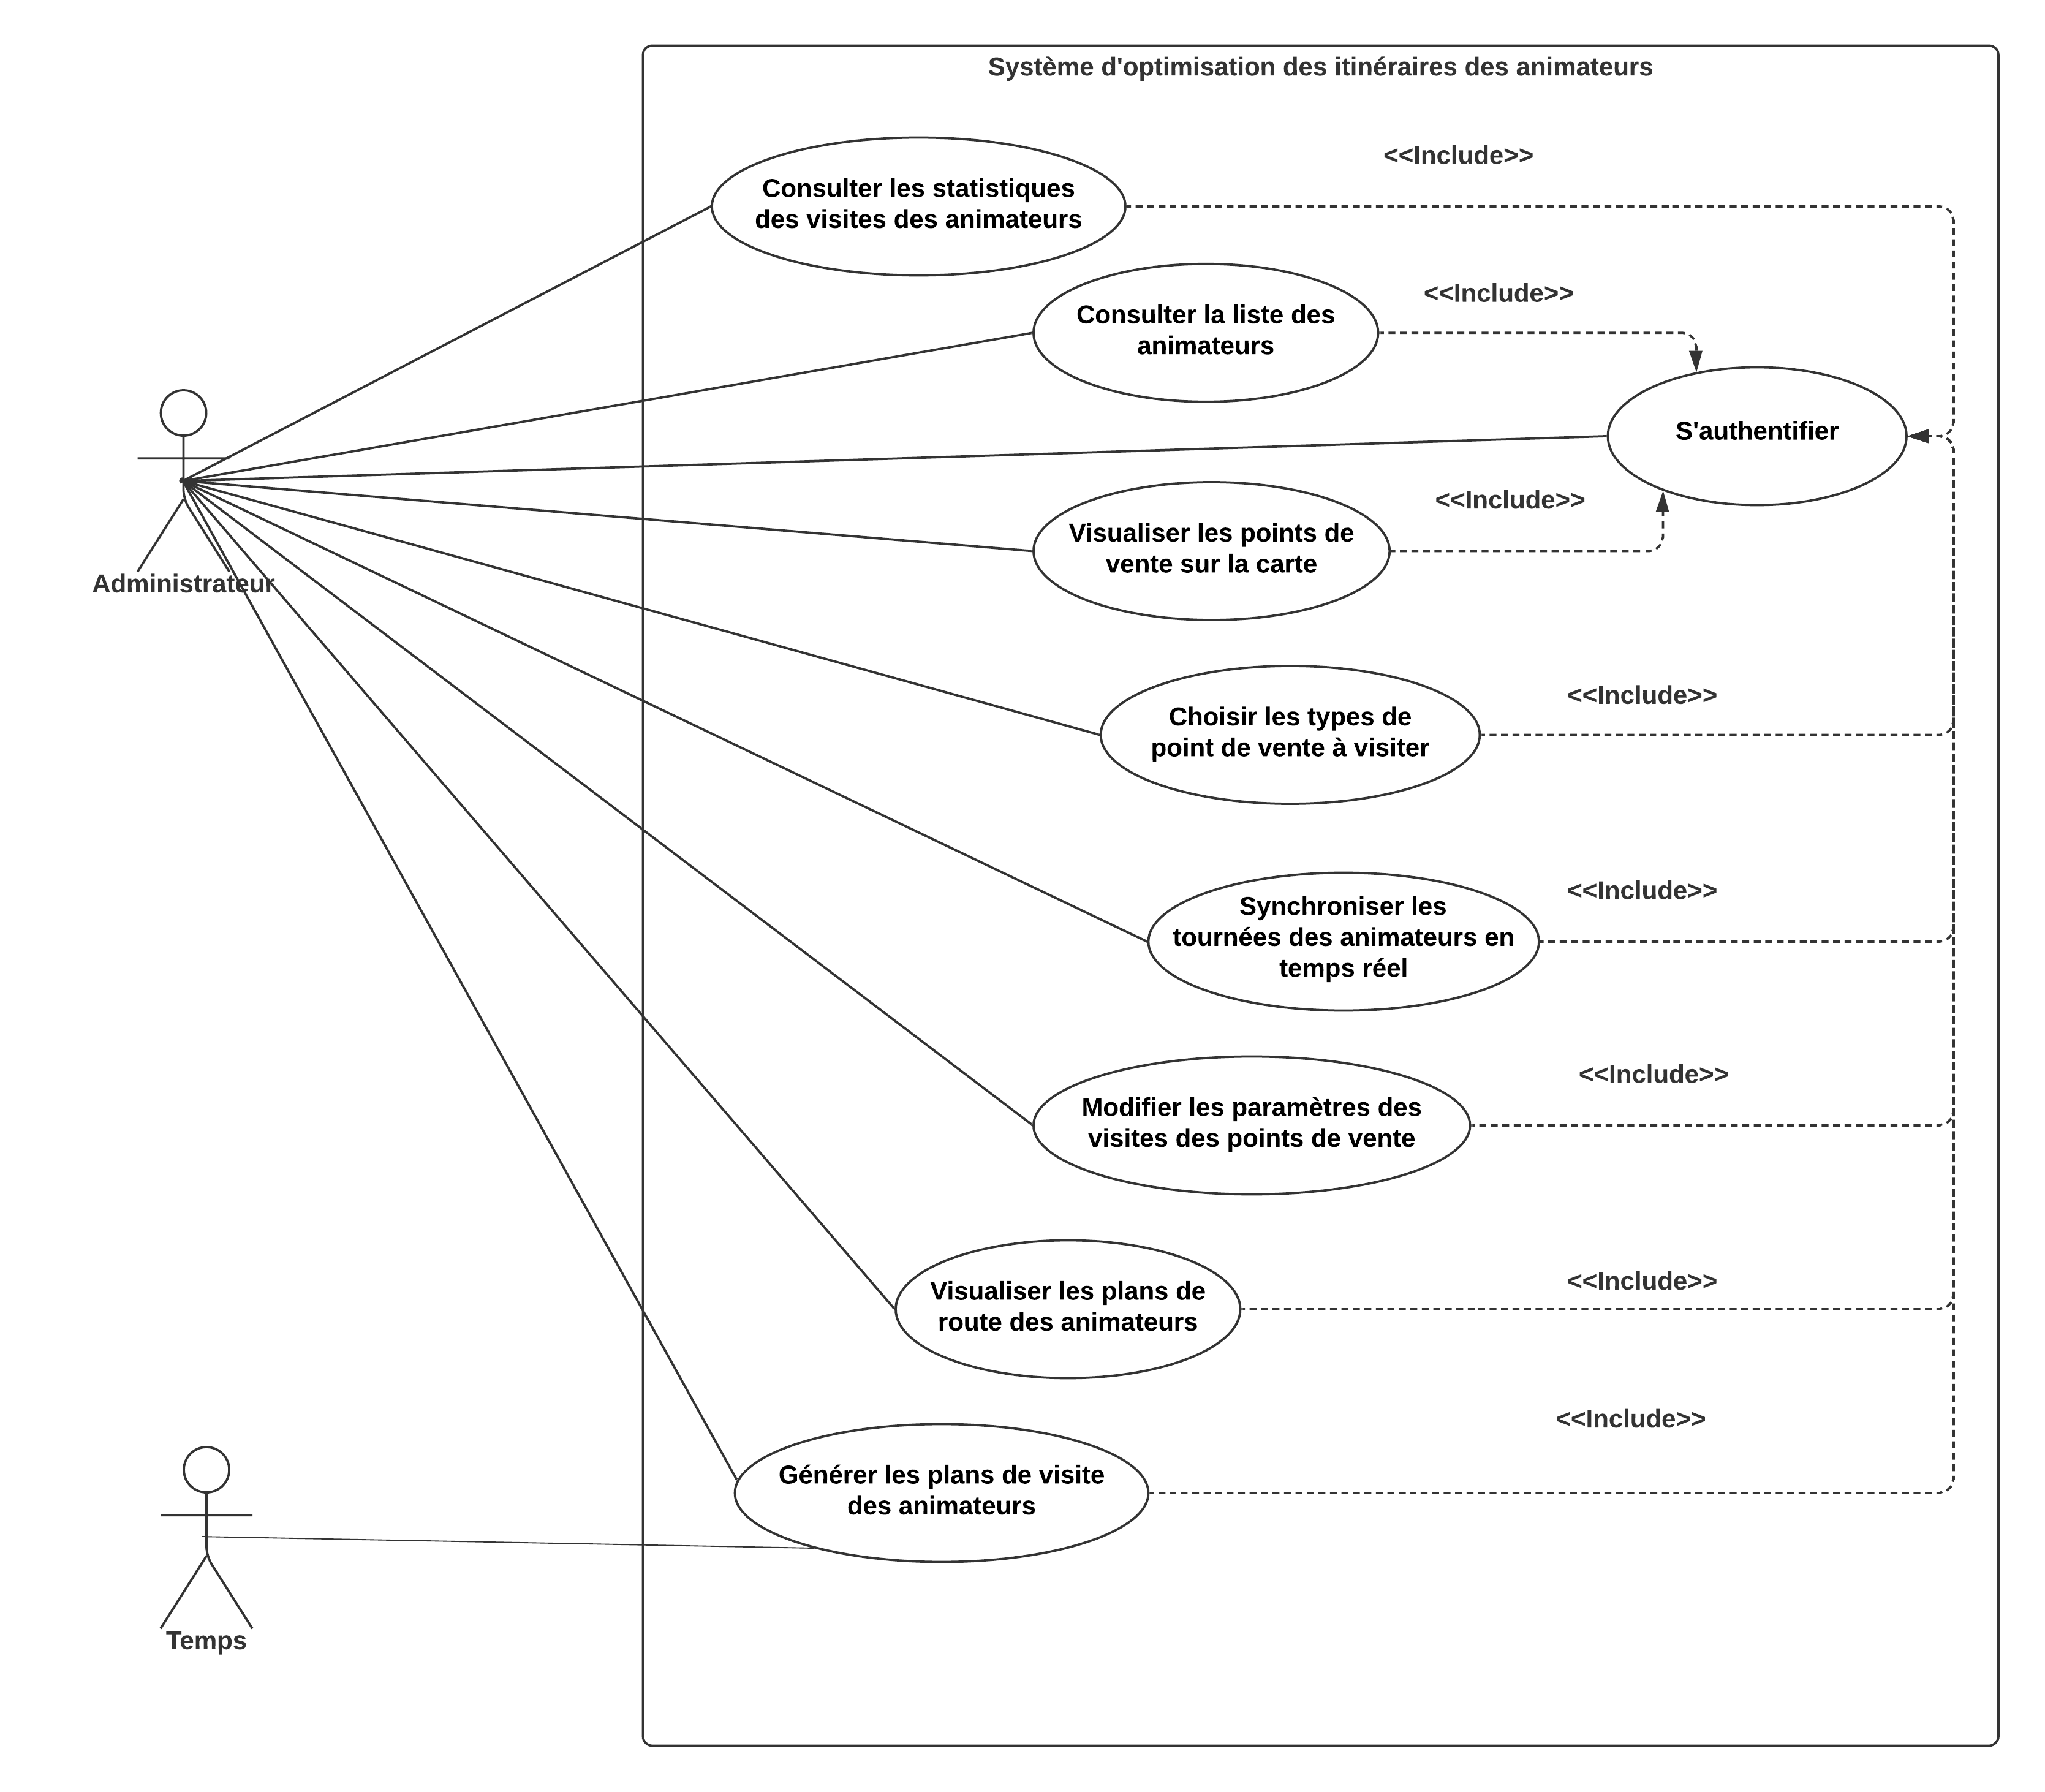
\includegraphics[ width=\linewidth]{images_pfe/DCU_ADMINISTRATEUR.png}
  \caption{Diagramme des cas d'utilisation de l'administrateur.}
  \label{fig:dcu-administrateur}
\end{figure}
\FloatBarrier


\renewcommand{\arraystretch}{1.5}
\begin{xltabular}{\linewidth}{|c|X|c|c|}
    \hline
    ID & CU & Documentation & Diagramme d'activité     \\\hline
    1 & S'authentifier & & \\ \hline
    2 & Consulter les statistiques des visites & & \\ \hline
    3 & Consulter la liste des animateurs & & \\ \hline
    4 & Visualiser les points de vente sur la carte & & \\ \hline
    5 & Générer les plans de visite des animateurs & \checkmark & \checkmark \\ \hline
    6 & Synchroniser les tournées des animateurs & \checkmark &  \\ \hline
    7 & Visualiser les plans de route des animateurs &  &  \\ \hline 
    8 & Modifier les paramètres de visite des points de vente & \checkmark &  \\ \hline
    9 & Choisir les types de points de vente à visiter & & \\ \hline
    \caption{Liste des cas d'utilisation de l'administrateur.}
    \label{tab:admin-use-cases}
\end{xltabular}
\FloatBarrier


\renewcommand{\arraystretch}{1.5}
\begin{xltabular}{\linewidth}{|X|}
    \hline
    \textbf{CU} : Générer les plans de visite des animateurs     \\\hline
    \textbf{ID} :  5   \\\hline
    \textbf{Description brève} : Générer les plans de visite des animateurs avec les chemins optimaux de parcours  \\\hline
    \textbf{Acteurs primaires} : Administrateur, Temps     \\\hline
    \textbf{Acteurs secondaires} :  /    \\\hline
    \textbf{Pré condition} :  l'administrateur déjà connecté    \\\hline
    \textbf{Enchaînement principal} : \\
    Le cas d'utilisation démarre automatiquement de manière périodique, ou lorsque l'administrateur souhaite générer les plans de visite des animateurs. \\
    1. L'administrateur choisit l'onglet génération des plans. \\
    2. Il introduit la période dans laquelle l'animateur va visiter les points de vente (semaine, 15 jours, mois...etc). \\
    3. Il choisit pour chaque type de point de vente sa fréquence de visite pendant la période. \\
    4. Il lance la génération des plans. \\
    5. Le système génère les plans de visite des animateurs. 
    \\\hline
    \textbf{Post condition} :  Les plans de visite sont générés pour l'ensemble des animateurs   \\\hline
    \textbf{Enchaînement alternatif} :   /   \\\hline
  
    \caption{Documentation CU : Générer les plans de visite des animateurs.}
    \label{tab:cu-specs1}
\end{xltabular}
\FloatBarrier

\clearpage

\renewcommand{\arraystretch}{1.5}
\begin{xltabular}{\linewidth}{|X|}
    \hline
    \textbf{CU} : Synchroniser les tournées des animateurs      \\\hline
    \textbf{ID} :  6    \\\hline
    \textbf{Description brève} : Mettre à jour une tournée d'un animateur par rapport à la fluidité du trafic routier     \\\hline
    \textbf{Acteurs primaires} :  Administrateur    \\\hline
    \textbf{Acteurs secondaires} :  /    \\\hline
    \textbf{Pré condition} :  l'administrateur déjà connecté   \\\hline
    \textbf{Enchaînement principal} : \\
    Le cas d'utilisation démarre lorsque l'administrateur souhaite synchroniser la tournée d'un animateur. \\
    1. L'administrateur choisit la section de synchronisation. \\
    2. Il choisit l'animateur en question. \\
    3. Il lance la synchronisation. \\
    4. Le système synchronise la tournée de l'animateur avec les données du trafic.
    \\\hline
    \textbf{Post condition} : La tournée de l'animateur est mise à jour     \\\hline
    \textbf{Enchaînement alternatif} :   /   \\\hline
    
    \caption{Documentation CU : Synchroniser les tournées des animateurs.}
    \label{tab:cu-specs2}
\end{xltabular}
\FloatBarrier


\renewcommand{\arraystretch}{1.5}
\begin{xltabular}{\linewidth}{|X|}
    \hline
    \textbf{CU} : Modifier les paramètres des visites    \\\hline
    \textbf{ID} :  8   \\\hline
    \textbf{Description brève} : Modifier les paramètres des visites des points de vente      \\\hline
    \textbf{Acteurs primaires} :  Administrateur    \\\hline
    \textbf{Acteurs secondaires} :  /    \\\hline
    \textbf{Pré condition} : L'administrateur est connecté     \\\hline
    \textbf{Enchaînement principal} : \\
    Le cas d'utilisation démarre lorsque l'administrateur souhaite de modifier les paramètres de visite dans le système. \\
    1. L'administrateur introduit la période des visites. \\
    2. L'administrateur introduit les fréquences de visite pour chaque type de point de vente. \\
    3. L'administrateur valide les paramètres.\\
    4. Le système enregistre les nouveaux paramètres.
    \\\hline
    \textbf{Post condition} : Les paramètres des visites sont modifiés     \\\hline
    \textbf{Enchaînement alternatif} :   /   \\\hline
    
    \caption{Documentation CU : Modifier les paramètres de visite.}
    \label{tab:cu-specs3}
\end{xltabular}
\FloatBarrier

\begin{figure}[hbt!]
  \centering
  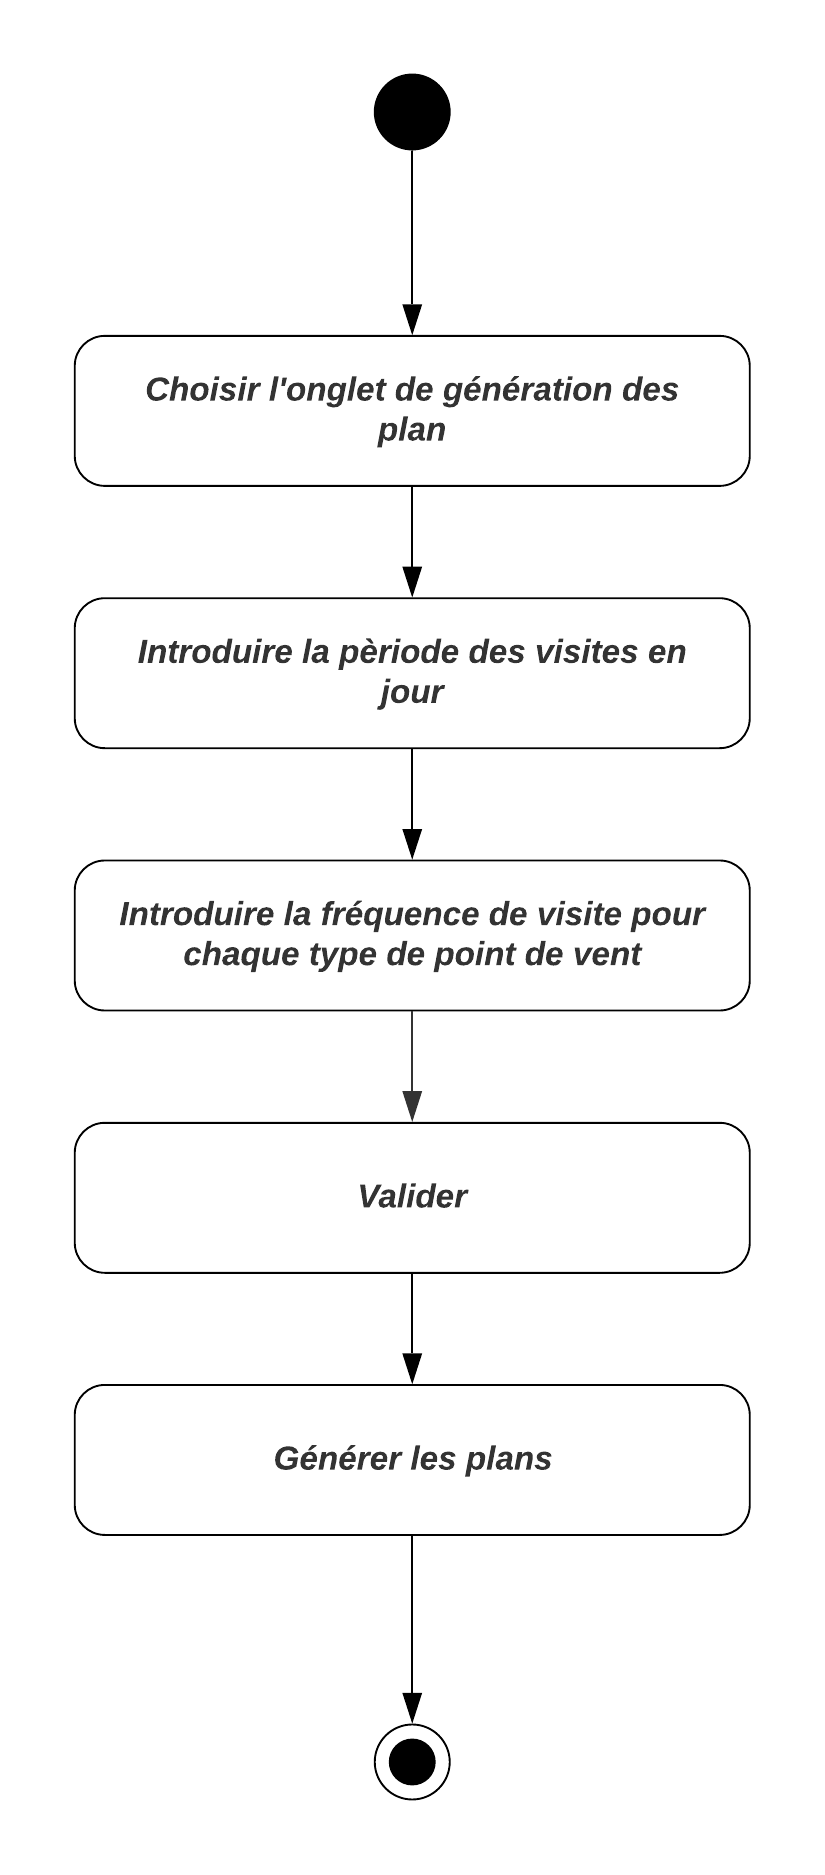
\includegraphics[height=17cm]{images_pfe/GENERATE_PLANS_DIAGRAM.png}
  \caption{Diagramme d'activité du CU: Générer les plans de visite des animateurs.}
  \label{fig:activity-admin}
\end{figure}
\FloatBarrier

\clearpage

\subsection{Animateur}


\begin{figure}[hbt!]
  \centering
  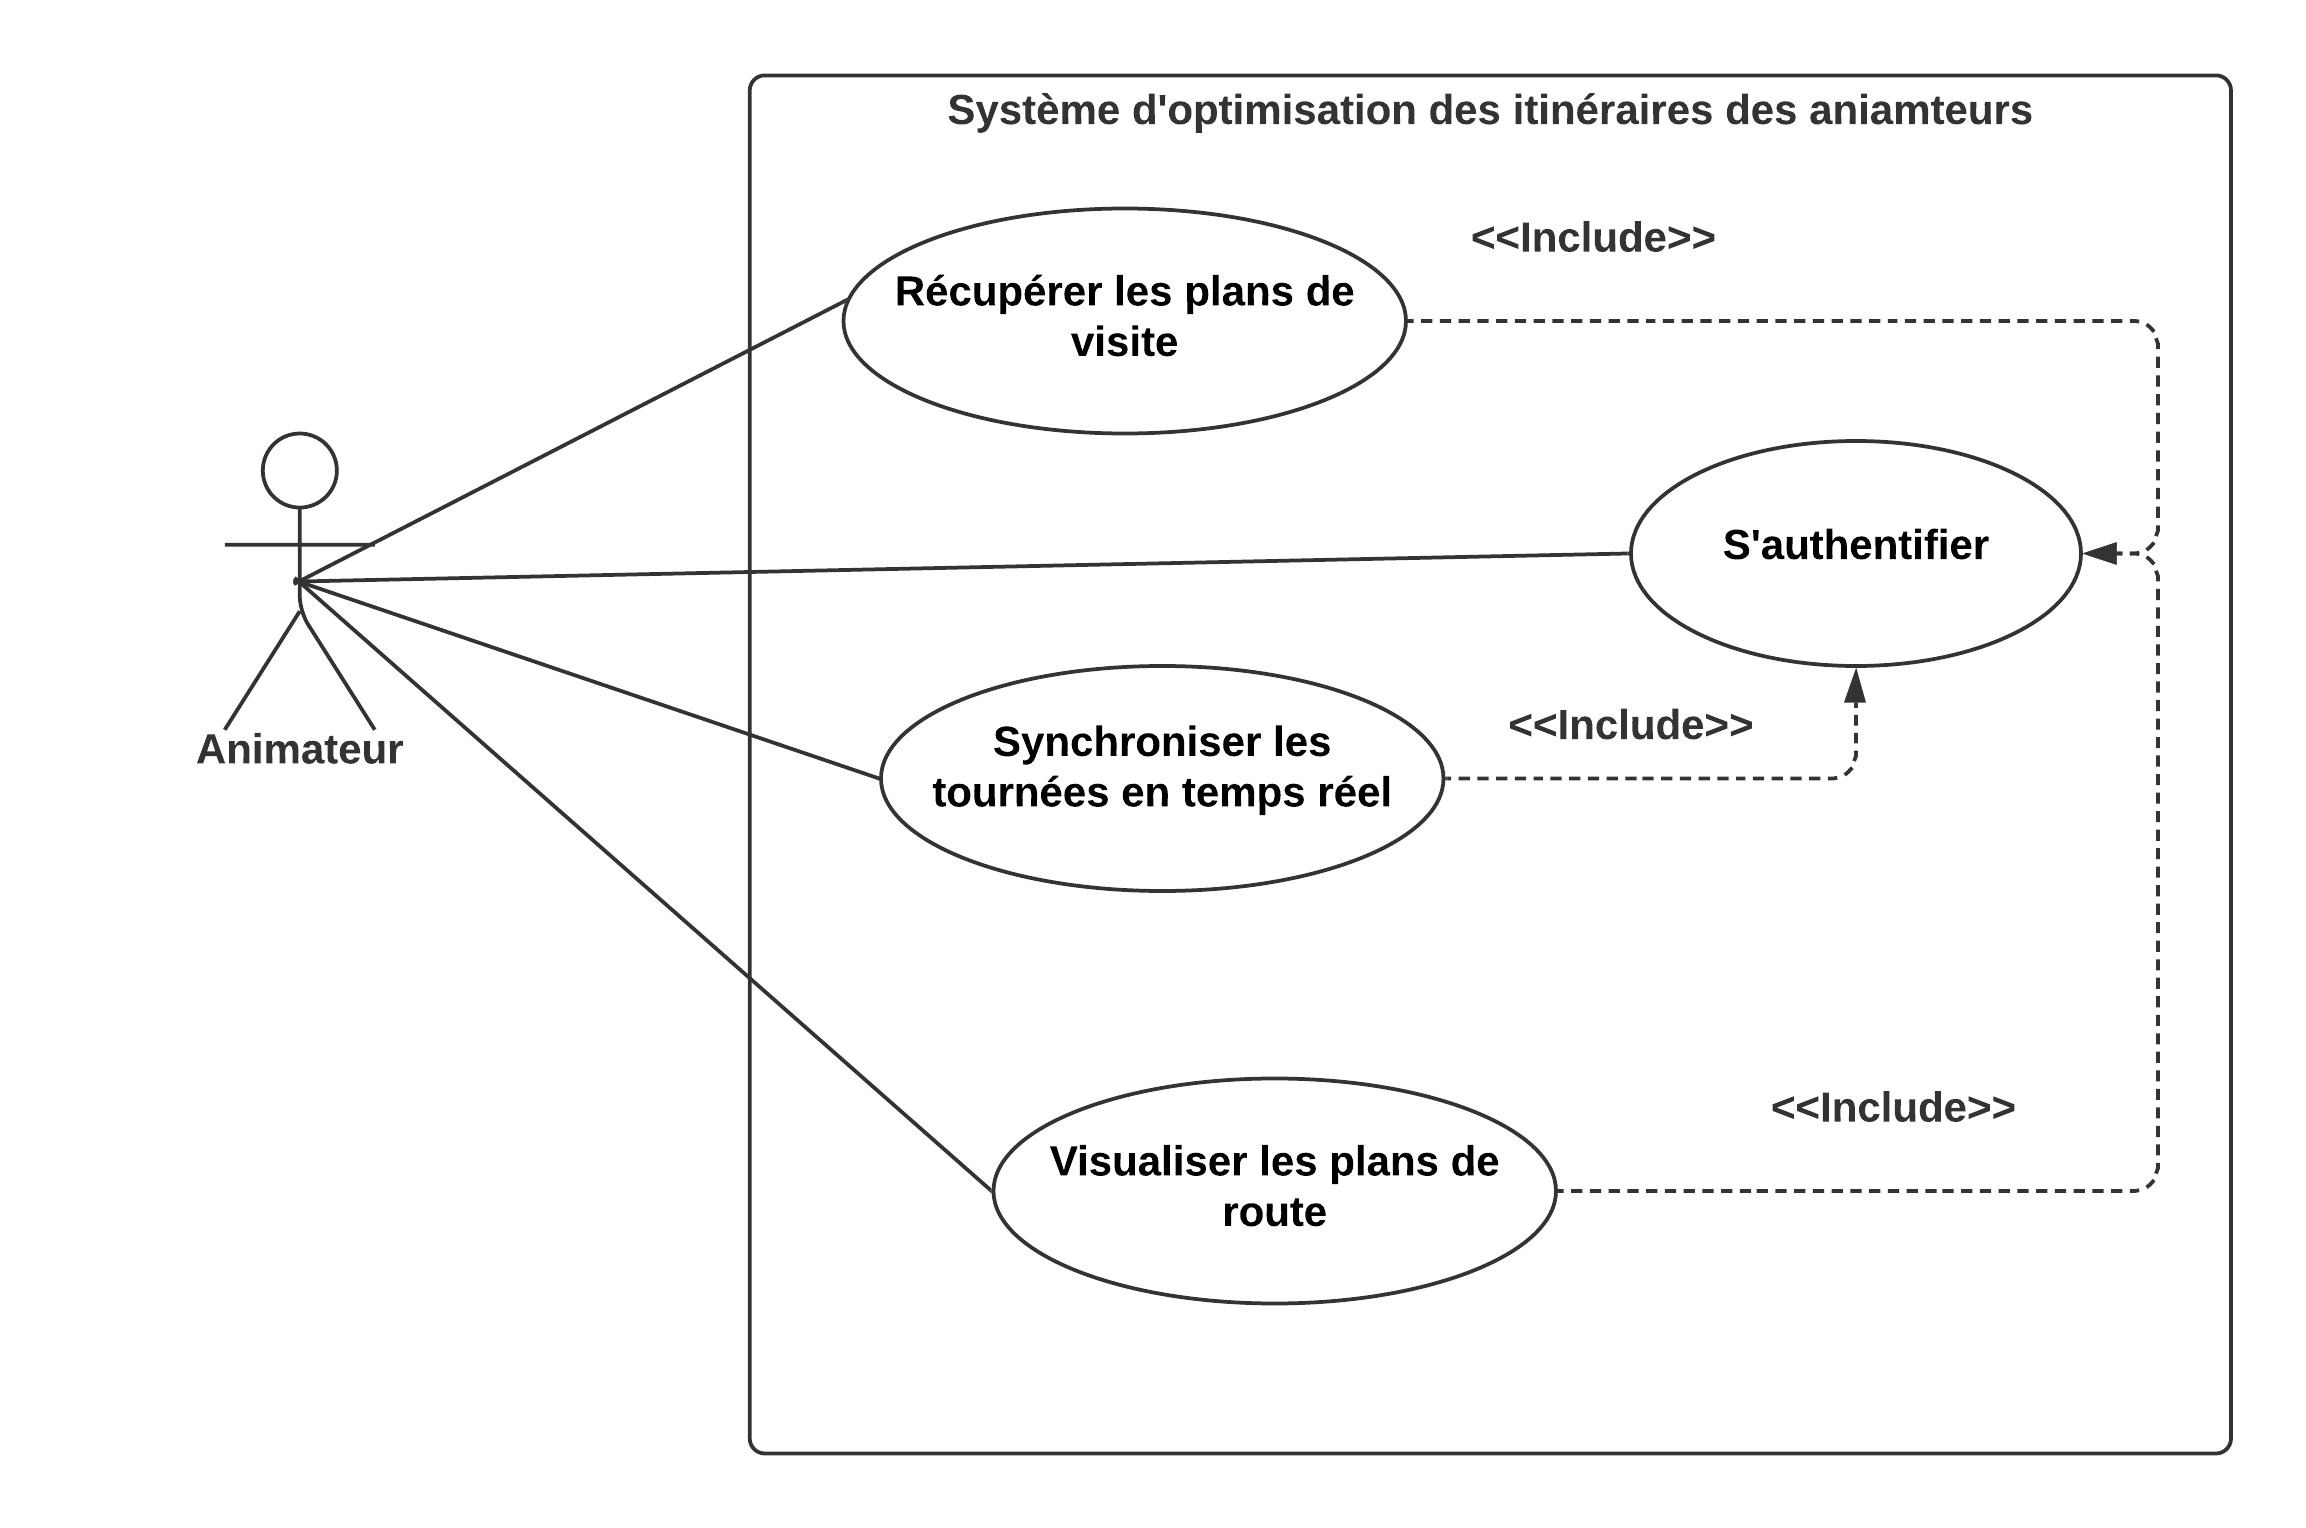
\includegraphics[width=\linewidth]{images_pfe/DCU_ANIMATEUR.png}
  \caption{Diagramme des cas d'utilisation de l'animateur.}
  \label{fig:dcu-animateur}
\end{figure}
\FloatBarrier

\renewcommand{\arraystretch}{1.5}
\begin{xltabular}{\linewidth}{|c|X|c|c|}
    \hline
    ID & CU & Documentation & Diagramme d'activité     \\\hline
    1 & S'authentifier & & \\ \hline
    10 & Récupérer les plans de visite & \checkmark & \\ \hline
    11 & Synchroniser les tournées & \checkmark & \checkmark \\ \hline
    12 & Visualiser les plans de route & & \\ \hline
    
    \caption{Liste des cas d'utilisation de l'animateur.}
    \label{tab:animator-use-cases}
\end{xltabular}
\FloatBarrier

\renewcommand{\arraystretch}{1.5}
\begin{xltabular}{\linewidth}{|X|}
    \hline
    \textbf{CU} : Récupérer les plans de visite    \\\hline
    \textbf{ID} :  10    \\\hline
    \textbf{Description brève} : Récupérer les plans de visite de l'animateur de pendant toute la période     \\\hline
    \textbf{Acteurs primaires} :   Animateur   \\\hline
    \textbf{Acteurs secondaires} : /     \\\hline
    \textbf{Pré condition} : L'animateur est déjà connecté   \\\hline
    \textbf{Enchaînement principal} : \\
    Le cas d'utilisation démarre lorsque l'animateur souhaite récupérer ses plans de visite.\\
    1. L'animateur choisit l'onglet plans de visite.\\
    2. Il lance la requête de récupération.\\
    3. Le système renvoie les plans de l'animateur.
    \\\hline
    \textbf{Post condition} :  Les plans de visite de l'animateur sont récupérés    \\\hline
    \textbf{Enchaînement alternatif} :  /   \\\hline
    
    \caption{Documentation CU : Récupérer les plans de visite.}
    \label{tab:cu-specs4}
\end{xltabular}
\FloatBarrier


\renewcommand{\arraystretch}{1.5}
\begin{xltabular}{\linewidth}{|X|}
    \hline
    \textbf{CU} : Synchroniser les tournées en temps réel     \\\hline
    \textbf{ID} :  11    \\\hline
    \textbf{Description brève} :  Mettre à jour la tournée par rapport à la fluidité du trafic routier    \\\hline
    \textbf{Acteurs primaires} :  Animateur    \\\hline
    \textbf{Acteurs secondaires} :   /   \\\hline
    \textbf{Pré condition} :   L'animateur est connecté   \\\hline
    \textbf{Enchaînement principal} :   \\
    Le cas d'utilisation démarre lorsque l'animateur souhaite synchroniser sa tournée.\\
    1. L'animateur choisit la section de synchronisation.\\
    2. L'animateur lance la requête de synchronisation.\\
    3. Le système renvoie la tournée synchronisée.
    \\\hline
    \textbf{Post condition} :  La tournée est synchronisée    \\\hline
    \textbf{Enchaînement alternatif} :  /    \\\hline
    
    \caption{Documentation CU : Synchroniser les tournées en temps réel.}
    \label{tab:cu-specs5}
\end{xltabular}
\FloatBarrier

\begin{figure}[hbt!]
  \centering
  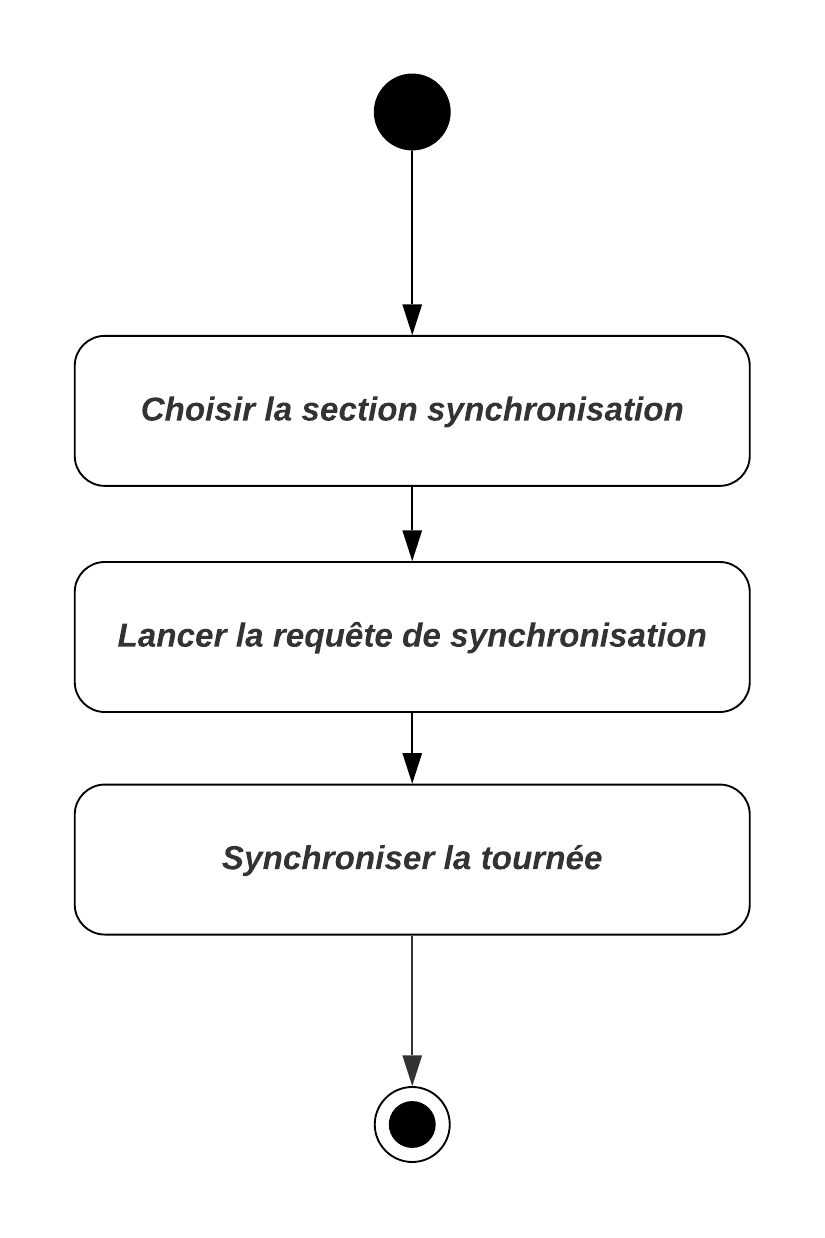
\includegraphics[height=13cm]{images_pfe/SYNC_TOUR_DIAGRAM.png}
  \caption{Diagramme d'activité du CU: Synchroniser les tournées en temps réel.}
  \label{fig:activity-animator}
\end{figure}
\FloatBarrier


\section{Conclusion}
Lorem ipsum dolor sit amet, consectetur adipiscing elit. Proin posuere euismod neque, non semper nibh viverra sed. Praesent ut varius magna. Fusce ipsum ante, semper nec interdum at, semper et lacus. Nulla ultrices magna a fringilla finibus. Etiam sollicitudin blandit ante. Vivamus blandit rhoncus tincidunt. Morbi sit amet congue purus. Praesent interdum gravida congue. Donec fermentum dui fermentum maximus rutrum.




%%% Local Variabs prles: 
%%% mode: latex
%%% TeX-master: "isae-report-template"
%%% End: 